\chapter{Head To Toe 3}

% \begin{figure}[H]
%     \centering
%     \includegraphics[width=\textwidth/2]{./Games/EveryChildCanSucceed/Images/EveryChildCanSucceed1CD.png}
%     \caption{Every Child Can Succeed 1 CD}
% \end{figure}

The third of the Head To Toe games published and released by The Lightspan Partnership for the PlayStation 1.

Head To Toe 3 features four video programs:

\begin{itemize}
    \item Control Center
    \item Fighting Germs and Diseases
    \item Sounds
    \item Sights
\end{itemize}

\clearpage
\newpage

\section{Control Center}

\subsection{Audio Summary}

"Control Center" describes the brain and the five senses that it controls: sight, hearing, smell, taste, and touch. It also describes how the brain is protected.

\subsection{Transcription}

Arnell: Okay, are you ready?

Louisa: Ready.

Arnell: Tell us what this is.

Louisa: Um, a feather?

Arnell: Are you sure?

Louisa: It's a feather! It's a feather!

Arnell: Correct.

Christopher: Can you tell us what this is?

Louisa: A music box.

Christopher: Yep.

Arnell: Tell us what this is.

Louisa: I think it's a banana.

Arnell: And\dots

Louisa: And what?

Arnell: Open your mouth. Take a bite.

Louisa: A bana- A banana with peanut butter on it.

Arnell: Correct.

Bob: Well how did Louisa know that it was a feather or a music box or a banana with peanut butter on it? Well, that's because she could feel, she could hear, she could smell, and she could taste. Do you know what those things are? Those are our senses, and we have five of them. We have taste, we have smell, touch, hearing, and sight. And you might want to try what the kids were doing where you cover your eyes and see if you can identify things just by touching them or smelling them or tasting them, and you'd be surprised just how much your five senses tell you about the world.

(video plays)

Male Singer: What part of you hears the ocean roar and the sound of rain as it starts to pour? What part of you hears your uncle snore? That's what your ears are for. That's what your ears are for. Won't you come and sing along, learning all day long, singing the senses song? What part of you can touch and explore the fur on a cat or the sand on the shore? What feels softness and sharpness and more? That's what your skin is for. That's what your skin is for. Won't you come and sing along, learning all day long, sing of the sense song? What part of you can see the colors from the back of a bee and the shape of a dinosaur? That's what your eyes are for. What part of you would just adore to taste an apple down to the core? And everything else in the grocery store? That's what your mouth is for. That's what your mouth is for. And what part of you just can't ignore the smell of bread behind the oven door? What part of you smells smells galore? That's what your nose is for. That's what your nose is for. Won't you come and sing along, learning all day long, singing the sensor song.

(back to the house)

*phone rings*

Bob: I'll get it. Hello? Ah, just a moment. For you Bird.

Bird: Thanks Bob.

Bob: Hang on. You know what this is, right? It's a telephone, and it can help us think about how our five senses work. When I speak into the telephone, my voice goes in here, right? But does it stay right there? Well, of course not. It becomes a message that goes down this cord and then it goes into another cord that goes into the wall, then through a whole bunch of other cords all the way across town until it gets to the person on the other end, and they get the message. Well the same kind of thing happens in your ear.

(video plays)

Bob (voice over): The sound goes into your ear and your ear sends a message along a kind of cord. The cord in your body is called a nerve. Where do you think these nerves go? To your brain. That's the place inside of your head that controls your body. Your brain gets the message that you're hearing something. It works the same way with all of your senses: hearing, taste, smell, sight, and touch. When you taste some food with your mouth, the taste doesn't stop there. Your mouth sends a message along nerves straight to your brain. When you smell something with your nose, or see something with your eyes, or touch something with your hand, or feel something with your foot, all of those messages are sent to your brain through nerves.

(back to the house)

Bob: And the nerves end up here in your brain.

Arnell: That's in my head?

Bob: Yeah, it's hard to believe, isn't it? Your brain is kind of folded on itself and wrinkled, and it's actually spongy and kind of soft, but it sits in your head just like this.

Arnell: Cool.

Bob: Yeah. This brain's a little bigger than a real one just so that we can see it. Actually, Larry over here can show us what the brain really looks like in the head. Let's suppose that Larry has a splitting headache today, okay. We can cut his head right down the middle and inside there's the brain. Can you see how it completely fills the top part of the head there. And part of the brain goes down the back, and these are nerves that connect in your neck. So those go down like this, they go down your neck and then they go through some other nerves that are down your back. It's ticklish 'cause there are a lot of nerves there. And the messages from your senses come in here at the bottom of your back. Now what do you think that your brain does with all those messages it gets from your senses?

Arnell: I don't know.

Bob: Well, let's suppose that we're going to go for a walk in the woods. Okay, so let's start walking through the woods. Nice day, having a good time. All of a sudden your ears hear some rustling in the leaves, and your eyes see a little black animal with a white stripe down its back, and your nose smells something really awful.

Arnell: I'm in trouble.

Bob: Well, your brain takes these senses in and thinks about them really fast. And what's it decide?

Arnell: I found a skunk.

Bob: A skunk! So quickly your brain takes those signals and sends new messages on other nerves back down to your body to tell it what to do. And your brain tells your legs to start running. Start running, legs! And your brain tells your arms to start pumping. Pump hard! And your brain tells your lungs to start breathing hard. Yeah, so you can get lots of oxygen, and\dots

Arnell: I'm outta here! *runs off*

Bob: Yeah! Well the important thing is that your brain takes messages from your senses, thinks about them, and then sends other messages back to your body to tell it what to do. Your brain is kind of like a control center, and it controls everything that you do.

(moves to another room)

Bob: Now I wonder, when you're walking through a forest and you see a skunk, how do you know that it's a skunk? I mean, that may seem like a silly question, but why don't you say, "Hey, there's an elephant," or "Hey, there's my bicycle"? Well, that's because you know what a skunk looks like - your brain remembers it. Maybe, maybe you've seen a picture of a skunk, or a drawing like this. Maybe you've seen a live one at the zoo or on the side of the road. So your brain remembers what a skunk looks like so you'll know it when you see it. Now your brain doesn't remember everything. I mean I'm always forgetting where I left my pencil. Do you forget things sometimes? Well that's okay, everybody does it. But what your brain remembers is amazing. I mean, you remember the letters of the alphabet, you remember that this is a baseball, you remember that this is a hat. You know the names of your family and your friends, and that list just goes on and on and on, and that's because remembering is the most important thing that your brain does.

(moves to another room)

Bob: You know that everybody's brain is special, and your brain might be special at some things like arithmetic or spelling, and other people are special in other things. For example, I know that Arnell's brain is really good at something.

Arnell: What?

Bob: Drawing.

Arnell: Oh yeah, I try to remember things and then I try to paint them.

Bob: That's right. Louisa, what do you think your brain's really good at?

Louisa: Well I like to read, and I like to play games.

Bob: But I also know that you like gymnastics.

Louisa: But does my brain do that?

Bob: Absolutely. Your brain is really good at controlling everything that your body does. Well, Naomi has a friend who's really talented, and she showed us how her brain helps her do amazing things.

(video plays)

Naomi: Hi, this is Naomi and I'm here with Karen in Karen's room and Merlin, her dog. Hi, Karen.

Karen: Hi.

Naomi: Karen, what is cerebral palsy?

Karen: Well, cerebral palsy means that the brain was damaged at birth, usually because not enough oxygen, and so the brain doesn't give the right messages to the muscles and it affects some things. It's hard for me to use my arms or legs, but it doesn't affect my thinking.

Naomi: I can't believe you're only 16 and you're writing books. What kind of books do you write?

Karen: Well, I've written a children's book about Merlin and how he helps me, and I've also written a mystery novel.

Naomi: Where do you get your ideas?

Karen: Well, just anywhere. A lot of times people I know will become characters in my books and ideas that I think of, or that, of things that I see and hear.

Naomi: What other things do you write?

Karen: Um, well I write for the school newspaper which is called the Whole Press, and I also have written some essays and short stories.

Naomi: Do you have any problems getting around at school?

Karen: Sometimes. They've done a lot to help people with disabilities at school by making things more accessible. But a lot of times it's hard because people who aren't in wheelchairs don't know what to do around people who are.

Naomi: How does Merlin help you at school?

Karen: Well, he carries my books for me.

Naomi: How does he help you around the house?

Karen: Well, he's trained to retrieve things that I drop because I can't reach the floor when I'm in my wheelchair. And he can go and get my mom if I need her. He opens the door for me, turns lights on and off, all kinds of things.

Naomi: How was Merlin trained to do these things?

Karen: Well, he was trained by Canine Companions for Independence in Ohio, and they especially train dogs to assist people who have disabilities. Merlin knows about 70 commands.

Naomi: How do you write with your computer?

Karen: My computer has a special program that can recognize my voice. If I say a word, the computer actually can hear it and understand, and then it prints it on the screen. And this helps because it's hard for me to type things that are long because my hands get tired.

Naomi: Why do you think you're such a good student? You've won all kinds of awards and everything.

Karen: I don't know. I work hard and I want to accomplish things, so I just work hard.

(Back to the house)

Bob: So your brain is a pretty wonderful thing. It lets you think, it lets you learn, it lets you use your senses. Now what do you think would happen if your brain was hurt somehow? Well, you may not be able to learn or think or use your senses as well as you can use them right now. You know, this model of the brain that we've been using here is actually made of plastic, and it's kind of hard. If you were to hold a real brain in your hand, it would actually feel quite different. It would feel sort of soft and squishy. A real brain is about as soft as pudding. Plop. And that soft brain needs to be protected. So where does your body protect it? Well, Mr. Bones can show us that. Hi, Mr. Bones. Nice hat. Your brain is protected by a very hard bone at the top of your head called your skull. And you can feel your skull if you just tap your head lightly on the side. You feel how hard it is there, and it's hard all the way around your head - a hard skull protecting a soft brain. And it's important to protect our brains because if you hurt your brain, it's very difficult to make it healthy again. And we need healthy brains because\dots

(video plays)

Bob (voice over): There are five senses: hearing, taste, smell, sight, and touch. Your sense organs send messages along cords called nerves. The nerves carry the messages to your brain. Your brain can think. It also sends messages back to your body. It's your control center. Your brain remembers things. Because you can remember, you can learn. Every brain is special and needs to be protected.

(back to house)

Bob: Come on, hey come on Christopher!

Louisa: [inaudible] You can do it!

Bob: The time is running out, is he going to do it? Is he going to make it? He's in the home stretch now! Here he comes! Oh, it's getting close and\dots Yay! Okay, well that was pretty good, Christopher, but now do you think you can do it again faster than that?

Christopher: I'm sure I can.

Bob: Okay. [inaudible]. Oh look at him go this time! Look at how fast he is! Yeah, whoa! Look at that! New world record! Yay! Now that's using your brain. Okay, Louisa, do you want to try one too? Here, let's see if you can do another one. See if you can get the, get across the river. Okay, this is another\dots

\subsection{Credits}

Models Donated by: Frey Scientific Inc, Denoyer-Geppert Science Company;
Footage Provided by: General Learning Video, Indiana State Department of Health, United States Olympic Committee, WTNO;
Special Thanks to: Bob, Kristen and Kern Willison, Wayport Pet Supply;

\section{Fighting Germs and Diseases}

\subsection{Audio Summary}

"Fighting Germs and Diseases" is about how germs enter the body to cause illness, and what children can do to stay free of disease.

\subsection{Transcription}

Shauna (acting): Don't touch that dial! It's time for your favorite show: The Attack of the Invisible Invaders.

Sam (acting): Sparky, we're being attacked by invisible invaders!

Chao (acting): You mean space aliens?

Sam (acting): No, worse than space aliens.

Chao (acting): You mean ghosts?

Sam (acting): No, we don't believe in ghosts. These invisible invaders are for real.

Chao (acting): You mean\dots

Sam (acting): Yes, Sparky, we're being attacked by -

Chao (acting) and Sam (acting): Germs!

Shauna (acting): Be sure to tune in next time when Sparky says -

Chao (acting): I don't feel so good.

Shauna (acting): The end.

Bob: Bye, have a good flight. Say goodbye Bird. Attack of the Invisible Invaders? It sounds like some kind of scary movie. But you know, invisible invaders really do exist. We call them germs. And germs are so small that you can only see them through a microscope. Germs float through the air, they land on your furniture, they cling to your drinking glass. They even land on your skin. Germs are everywhere, and it's important that we think about germs because if they get inside your body, you can become really sick, and we all know that getting sick isn't much fun. So let's have a look through the microscope and see what these tiny germs really look like.

(video plays)

Bob (voice over): Germs are alive. If germs like these get into your body, you might get the flu. Germs may give you a runny nose, sore throat, make you sneeze and cough so you have to stay home from school.

(back to the house)

Bob: These germs can get into your body and make you sick, but how do they get in there? I mean your skin covers most of your body and it protects you against germs, but your skin doesn't cover everything. It has holes in it. In fact, I hate to tell you, but you've got holes in your head.

Shauna: Bob, that's not a very nice thing to say.

Bob: Well it's true Shauna, you do have holes in your head. What do you listen with?

Shauna: My ears.

Bob: Aha, two big holes right in the side of your head. What do you speak with?

Shauna: My mouth.

Bob: Aha, another big hole right in the front of your face.

Shauna: And my nose is another hole.

Bob: Right. So we've got three holes right there; three ways that germs can get in. But what do you do? I mean you can't, you can't cover your ears and close your mouth and plug your nose forever. So how do we protect ourselves against those germs?

(video plays)

Shauna (acting): And now it's time for the Attack of the Invisible Invaders part two.

Sam (acting): Sparky, the invisible invaders are all around us. They're on my microphone, they're on my juice glass, they're floating in the air. We have to stop them before they enter our bodies, but how? Sparky, what are you doing?

Chao (acting): No germs can attack me in here!

Sam (acting): There has to be an easier way.

(back to the house)

Bob: Well Sam's right, germs are everywhere, but you don't have to wear a rubber suit and a mask to keep them out of your body. There are other things you can do, things that are really easy. What do you think is the best way to protect yourself from germs? Should you clean your room, wash your hands\dots

Shauna: Or comb your hair?

Bob: What do you think is the best way to keep germs out of your body? You decide. Well, what did you decide? Shauna, do you know the answer?

Shauna: Wash your hands.

Bob: Right.

(video plays)

Bob (voice over): When you wash your hands, you can see that dirt gets cleaned away. But what you don't see is that most of the germs on your hands get killed. That's because soap and water kill germs, and your hands can have a lot of germs on them. Why? Because we use our hands for everything.

Male singer: Hello ladies and germs! And speaking of those cuckoo nutty little wacko germs, nobody wants 'em. So here's a little tune about what you can do to get rid of them. What you going to do today? What things will you make? What games will you play? Whatever you choose, you're probably going to use your hands. Are you're gonna to tie your shoes? Will you comb your hair? Will you read the news? Even just reading, buddy you'll be needin' those hands. You might clean up your bedroom or go dig around for worms. But did you know that much of the world is positively crawling with germs? What you gonna to do tonight? Will you help make dinner? Were you sitting right? No matter what is done, understand if you want to squash those germs, by gosh, whenever you can, just hear me, man. You're going to have to wash, wash those hands. Scrubby dubdub.

(back to the house)

Bob: Every time you touch something, there's a chance that germs get onto your hands. So then when you touch your face, like around your eyes or your nose or your mouth, those germs could get into your body. But if you wash your hands with soap and water, that kills a lot of the germs on your hands, so there aren't as many of them to get into your body. And there are some other things you can do as well. Suppose you're outside playing and you fall down and you cut yourself. You know, I mean, it happens all the time. You scrape your knee. Well, that cut becomes another hole in your body. So if you wash the cut with soap and water, then that can prevent germs from getting in. Here's something else. Suppose you're thirsty, you'd like a drink? Go over to the sink and you see a glass sitting there. But other people have been drinking from this glass before you. Should you take a drink from it? Yes or no? Well, the answer is no. The people who drank from this glass before you left germs around the rim, so when you drink from it, those germs can go into your mouth and into your body. So wash the glass before you drink from it. One more thing: suppose a friend of yours got a really nice, big lollipop and has been licking it away, and they offer you a lick. Should you lick the lollipop? Yes or no? Uh-uh. Even though you can't see them, the germs are there, and they could make you sick. But you know something? Oh, hi, Mr. Bones. Nice mask. Your body is very, very good at fighting germs.

(video plays)

Bob (voice over): Inside of your body are millions of special cells, a tiny army of germ killers that live in your blood. When germs get into your body, these special cells find the germs and attack them.

(back to the house)

Bob: These germ killers are always at work trying to keep you healthy, but sometimes they can't kill the germs fast enough, and well, that's when you get sick. So what happens then? Well that's when your doctor or your parents give you medicine.

(video plays)

Bob (voice over): Some medicines are germ killers too. They find the germs, attack them, and soon you feel better.

(back to the house)

Bob: Shauna has some pictures of different kinds of medicines. So Shauna, who's the guy in the picture?

Shauna: That's my friend Joey.

Bob: Ah, so where are his medicines?

Shauna: Well sometimes when you're sick, you have to take pills, and sometimes the medicine is in a bottle.

Bob: When it's a liquid.

Shauna: Uh-huh. You take it with a spoon. This really isn't medicine, but when you're sick, getting rest is good because that helps kill germs too. And sometimes you have to go to the doctor, and he gives you a shot.

Bob: Do you like getting shots?

Shauna: No, I hate them.

Bob: Why?

Shauna: Because they hurt.

Bob: Oh. Well, sometimes they sting just a little bit, but that's only for a moment. Then the germs are killed faster, and you feel better that much quicker. So what's your last picture?

Shauna: That's Joey.

Bob: Joey? Where?

Shauna: Well, he got a shot, so he felt better, and he went out to play.

Bob: I should have known. You know, before we had medicine, kids got sick a lot more than they do today. Without the medicine, they got things like measles and mumps and whooping cough, and almost anybody could get those diseases. But today, we have super special germ killers, and they keep you from getting those diseases. Well, our friend Sarah went to the health clinic, and she got some of those super special germ killers.

(video plays)

Sarah: But Dad, I'm not sick!

Dad: I know you're not sick.

Sarah: So why do I have to go to the doctors?

Dad: Sarah, sometimes we have to go to the doctors even when we're not sick.

Sarah: Why?

Dad: I'll let the doctor tell you.

Sarah: Okay.

(next scene)

Doctor: Say "ah."

Sarah: Ah. I'm not sick.

Doctor: Oh, I know you're not sick. In fact, you look very healthy.

Sarah: So why do I have to go to the doctors?

Doctor: Well, we don't want you to become sick. A long time ago, kids used to get spots all over their face and cough, or their neck and face would get very swollen, or sometimes they couldn't even walk.

Sarah: Could that happen to me?

Doctor: Well it could, but today we're going to give you a vaccine so that you don't get sick. The vaccine is in the form of a shot. Do you want a shot, or do you want to take a chance on getting sick?

Sarah: I think I want to have the shot.

Dad: I think you made a very good choice.

Sarah: I know I did.

(next scene)

Bob (voice over): Invisible invaders called germs are all around you. They can get into your body. You get a lot of germs on your hands, but soap and water kills germs, so the best way to fight germs is to wash your hands often, especially before you eat and after you go to the bathroom. And never put objects into your mouth or anything that other people have put into theirs. If germs get into your body, they're attacked by germ killers in your blood. Medicines also help kill germs in your body. Special medicines called vaccines can keep you from getting the measles and other terrible diseases.

(back to the house)

Chao (acting): Ooh, this is terrible! This is horrible! This is the worst thing in the history of the universe!

Sam (acting): What, Sparky, what?

Chao (acting): I cut my finger! What should I do?

Sam (acting): You should know that by now.

Chao (acting): Oh yeah! You drive.

Shauna: Will Sparky be okay? What should he do to the cut on his finger to protect him from 'The Attack of the Invisible Invaders?' Do you know?

\subsection{Credits}

Models Donated by: Frey Scientific Inc, Denoyer-Geppert Science Company;
Special Thanks to: Riviera Medical Center (Dr Patricia Huse), Purdue University Department of Biological Sciences, Bloomington Hospital Labratory;

\section{Sounds}

\subsection{Audio Summary}

"Sounds" tell why and how ears can hear sounds, and the danger of loud sounds that can damage a child's ears.

\subsection{Transcription}

Bob: So are you ready Christopher?

Christopher: All set.

Bob: Christopher took his tape recorder and he recorded all kinds of interesting sounds, and he wants us to try to guess what they are. Okay.

Christopher: Listen.

Bob: That's easy: that's the sound of a clock.

Christopher: Uh-huh.

Bob: Okay. That's easy: that's a drip like out of a tap or a faucet.

Christopher: Yep, you're right.

Bob: Okay.

Christopher: You'll never guess this one though.

Bob: Gee, um, that sounded like somebody playing some kind of musical instrument.

Christopher: No, that was wind chimes.

Bob: Wind chimes? Wow, did you get that? Wind chimes. Wow, that was great Christopher.

Christopher: I've got some more.

Bob: Okay. There are so many different kinds of sounds, and they tell us so much about the world. Have you ever taken the time to just stop and listen?

Bob: Well, that was a siren. Was it a police car?.

Christopher: An ambulance.

Bob: Okay. well that's a piano. Do you play the piano?

Christopher: No, my brother does?

Bob: Oh, you just play the tape recorder, right?

Christopher: Very funny.

Bob: Sounds tell us so much about the world. Like the siren tells us to get out of the way, and music, well, it just makes us feel good. But have you ever wondered how do sounds happen, and how are we able to hear all of the sounds that are around us?

(video plays)

Bob (voice over): Sound begins when something vibrates. That means it shakes or quivers very fast, like this violin string. That vibration makes the air around it vibrate too. The vibrating bits of air, we've colored them yellow so you can see them, spread out in all directions. When the air vibrations reach your ear, they make parts of your ear vibrate, and that's when you hear.

(back to the house)

Bob: That was the sound of somebody playing a violin.

Christopher: Yep.

Bob: How many sounds did you get? Wow, that was a great sound Christopher. That was really realistic!

Christopher: But I didn't do that.

Bob: You didn't? Uh-oh.

(move to another room)

Bob: Is everybody okay?

Christopher: What happened?

Joy: We accidentally tied over the recycling bins.

Sarah: We were looking for these!

Bob: Tin cans?

Joy: We're going to make a telephone!

Bob: Oh, a tin can telephone! Oh, that's a great project!

Sarah: We'll clean up first.

Bob: Okay. Can Christopher help you work on it?

Sarah: Yeah.

Bob: Okay, you guys get busy there. Have you ever done that? Tried to make a telephone out of two tin cans and a string? It's a great thing to do because it really shows you how sound comes from vibrations. Now, while the kids are working on their telephone, that gives us a chance to think about what happens to those vibrations when they get inside your ears, and - oh, hi Mr. Bones. Nice earmuffs. When somebody says ears, what do you think of? These things, right? Well, here's a model of your ears, and it shows you what your ear looks like on the outside and on the inside. Now let's talk about the outside part first. Now the part of your ear that you can see on the outside of your head is called the outer ear because it's on the outside, and this part acts kind of like, well, like this. This is a cone, the kids made it, it's just out of paper, and when sound goes in here, it comes out the other end, and if I hold this up to my ears, I can hear much better now. I can hear the sound of the refrigerator motor, and I can hear the sound of the bird outside. Hello bird!

Bird: Hi Bob!

Bob: Would you like to try it? Let's do this. The kids are still working on their telephone way on the other side of the room. Can you hear them? Listen.

Christopher: Hello.

Sarah: [inaudible]

Bob: You can hear them a little bit, but they're kind of far away. Now let's try it with this. We'll bring down our microphone here so you can hear better. Now listen to what happens when I put the cone over top. What does it sound like now?

Christopher: [inaudible]

Bob: Can you hear them better now? Now listen to what happens when I turn it over this way. Can you hear them now? Not as well. You hear best when your ears are pointed right at the sound.

Joy: I'm going to the museum today. Are you going\dots

Bob: So that's how the outer part of your ear works, it sort of works like this cone to direct sound into your head. In fact, you can do this yourself. Try this right now: just take your hands, cup them like that, and put them behind your ears and listen. Can you hear better? In fact, I can hear my own voice better now because my hands are directing the sound into my ear. So that's why the outside of your ear is sort of shaped like a cupped hand, and it directs the sound where? Into a hole. And that hole goes here. Now sounds are vibrations in the air, and when they go into your ear, the first thing they hit is a drum. It looks like this, let me take this piece out. It's called your eardrum because it really looks like a little drum: it's round, and it has a very tight skin across the center, and when sound vibrations hit that, it vibrates up and down many times a second, really fast, and I can show you how that works. In fact, this is something that you can try yourself. I've taken a glass and attached some plastic wrap to it, and stretched it very tightly over the opening of the glass so that it's really tight like a drum; like your eardrum. Now when sound vibrations hit that, it will vibrate up and down, and just to show you what that looks like, let's put some salt on top of our drum, and that's just so that we can see how it vibrates when sound hits it. Now we need some sound. Let's see, here's a ukulele, we can use this. Watch what happens to the salt when I make a sound. Can you see how the salt vibrates? It dances around. That's because the surface of the drum is bouncing up and down, vibrating when the sound vibrations hit it - sort of dancing to the music. In fact, it'll also work with my voice. La la la la. Laaaa. So that's what happens when sound goes into your ear. The sound vibrations cause your eardrum to vibrate back and forth many times a second, like the salt was on the glass. Now attached to your eardrum are three very tiny little bones, they're actually the smallest bones in your body, and this is called the middle ear because it's kind of in the middle of your ear. And when your eardrum vibrates like this, those bones vibrate back and forth. The bones are attached to another piece called your inner ear 'cause it's farther in, and it's a round part right here that has liquid inside it. Now what do you think happens when these bones vibrate? What happens to the liquid? Well, the liquid's going to vibrate too, right? So in fact, your whole ear actually vibrates and moves back and forth every time you hear a sound. Now when that liquid moves inside, it touches a special nerve, and that nerve sends a signal off to your brain, and your brain says, "I hear a sound." And I hear a sound. I'll get it.

(moves to another room)

Bob: Oh hi, Bert! Come on in. Hi, it's good to see - Oh, I guess I should say, *with sign language* hi Bert. Um, is this for us? Oh, sorry, sorry, it's so heavy thank you for bringing it, oh, well I'll put it over here. Um, hey Bert? Do you have time to meet somebody? Sure? This is our friend Bert. He brings a lot of the neat things that come to this place. Oh, hi Joy.

Joy: Hi.

Bob: You two know each other?

Joy: Yes.

Bob: Oh wow.

*Bert signs to Joy*

Joy: Yes, I remember the signs you taught me. Watch. This is "bird", this is "river".

*Bert signs to Joy*

Joy: We are\dots We are going to make a telephone.

*Bert signs to Joy*

Bob: *bob signs to Bert* Um, we'll show you when it's finished.

*Bert signs to Bob*

Bird: Oh, okay.

Bob and Joy: Bye Bert, sorry you got to go.

Joy: I have to go to work on the telephone.

Bob: Okay, you go work on that with the other kids. Gee, I wonder what this is. Fun stuff. We'll have to open that later. Oh.

(video plays)

Bob (voice over): Do you hear all of the sounds around you? Are your ears okay? Well one of the ways that you can find out is to have your ears tested, and that's what Diego did last week.

Audiologist: And I'm going to put these on. We're going to do one ear at a time, and you're going to hear some different sounds, it's going to go kind of beep beep beep. When you hear the beep, I want you to just raise your hand for me, okay? This one real high. Okay, if you have any questions, you stop me. Okay, ready?

Diego: Yeah.

Audiologist: Okay, we're going to do the right ear first. Raise your hand when you hear the sounds for me. Good. Now it's going to get softer. Listen for this one. Good. Good. Now same thing in the other ear. Okay. Good job.

(next scene)

Audiologist: Okay, now this is a graph. Going across here on this graph are the pitches from low pitch to high pitch. Going down is loudness. Down to this black line is considered within normal. The red marks are his right ear, blue marks are his left ear. So it all looks very much within normal across the board at all the pitches. So everything looks very normal. Looks great. You did a good job.

Diego's Mother: Good.

Audiologist: Yeah. Do you have any questions?

(back to the house)

Bob: Well, Diego's hearing is very good, and that's great, but he still needs to protect his ears because if you don't protect your ears, you can lose your hearing, especially when it comes to things like loud sounds. So if you listen to music, especially the real boomy kind, if it's too loud, it can damage your ears. That's why people who work in loud places, they wear things like this. These are ear protectors, and they block out a lot of those loud sounds so the ears are not damaged. Did you know that you can damage your own ears? Every time you clean them, you should never ever stick anything like this inside your ear. This is a cotton swab. Now you can clean lots of things with these, but not your ears, because your eardrum, remember that little drum that's just inside your ear? Well, if you put a cotton swab in, it could push against that and it could damage your eardrum and damage your hearing. So if you're gonna wash your ears, do it with a cloth and just wash the outside of your ear and do it very gently. It's important to keep your ears healthy because\dots

(video plays)

Bob (voice over): The world is full of sounds. Sounds begin when something vibrates. Vibrations travel through the air to our ears. The ear has five major parts: the outer ear which you can see, the eardrum, three bones attached to the eardrum which pass vibrations on to the liquid in the inner ear, which sends a message through a nerve all the way to your brain. Some people are hearing impaired. Many of them use signs to communicate. You can have your hearing tested. Loud sounds might damage your ears, and never ever put anything inside of them.

(back to the house)

Joy: So what's in the box?

Bob: Well, I don't know. This is the box that Bert brought me, so let's see what it is in there. Ooh, look at that. Isn't that nice? That's a seashell. You know they say that you can hear the sound of the ocean in a seashell if you listen like this. Oh yeah. Can you hear something, Christopher?

Christopher: Yeah.

Bob: Isn't that neat? Maybe we can all try it later on.

Sarah: Bob, we got our tin can telephones ready.

Bob: You did? Okay, well then let's try it out and see how it works. Oh, really long string you've got on that. Okay.

Joy: Hello? Hello? Can you hear me? Does this thing work?

Sarah: I hear you. Can you hear me?

Joy: Yes, really loud.

Bob: Isn't that great? The phone really works! Now why do you think that the tin can telephone really does work? Well, now that you know something about vibrations, maybe you can figure it out.

Sarah: Bob?

Bob: Yes, Sarah?

Sarah: It's for you.

Bob: For me? Who's calling me here?

Joy: Hello?

Bob: I told you not to call me here. Did it work? Could you, could you really hear through that? Yeah, it really works through the string, doesn't it? Could you?

\subsection{Credits}

Models Donated by: Frey Scientific Inc, Denoyer-Geppert Science Company;
Special Thanks to: [Sabbitt] White, [Pugh and Sarra] Inc, Patti Shea (Audiologist);

\section{Sights}

\subsection{Audio Summary}

"Sights" is about the eye. It talks about how they work, and the different things children can do to help protect their eyes and eyesight.

\subsection{Transcription}

Bob: Woah. Oh hi Naomi, come on in. Hi. Chao and Sarah are already here. So what's new?

Naomi: What's different about me?

Bob: What's different about you? Uh\dots You have a new shirt?

Naomi: No.

Bob: No. Okay, you have a new pair of shoes?

Naomi: No.

Bob: No. Well, there is something different about you, but I can't quite see what it is. I know, you've got a new haircut!

Naomi: Bob!

Bob: Oh, you have new glasses! I didn't notice that. Hey everybody, come here! Look, Naomi's got some new pair of glasses. Isn't that neat?

Chao: Can you see better now?

Naomi: A lot better. Before, I had trouble seeing things far away.

Bob: Well how did you know what kind of glasses to get?

Naomi: I went to the eye doctor.

(video plays)

Optician: Okay Naomi, I'm going to have you hold this and I want you to cover up your right eye for me, and you see that chart out there? I want you to tell me the smallest row of letters that you can read. And take a guess, it's all right to guess.

Naomi: O H P L C.

Optician: Good job. Okay, now I want you to cover your other eye and I want you to do the same thing, tell me the smallest row of letters that you can possibly read.

(skip forward in the video)

Optician: Okay Naomi, I'm going to have you put these red-green glasses on. Okay, can you see those dots out there?

Naomi: Yeah.

Optician: Okay, I'm going to cover one eye, and tell me what's the number of dots and what color they are.

Naomi: Three and they're green.

Optician: Good. And what about now?

Naomi: Two and they're red.

Optician: Okay.

(skip forward in the video)

Optician: Now what we're going to have you do, I want you to look out in the distance for me and just keep looking out there. Good. I'm going to be shining this light in your eye. Just keep looking out there. Good.

(skip forward in the video)

Optician: Okay, now what we're going to do is put some lenses in front of your eyes, and you go ahead and sit back and see if these lenses will improve your vision any. What I'm going to have you do is look out at that chart. Can you see that [blurred] line?

Naomi: Yeah.

Optician: All right. I want you to tell me when that first gets a little bit blurry to you.

Naomi: A little blurry.

Optician: It's a little blurry? Can you make it out here?

Naomi: No.

Optician: No, okay. I want you to tell me when you can first see a letter on that line.

Naomi: I can see a letter.

Optician: Okay, does this improve it any?

Naomi: Yeah.

Optician: Okay. What about here? Or does it look the same?

Naomi: Um, it just looks the same.

Optician: Looks the same? Good. Okay, I want you to keep looking at that row of letters, and I want you to tell me which one looks better to you. One or two?

Naomi: One.

Optician: Good. Okay Naomi, what we're going to do now, if you look out through those lenses and then look out without the lenses, which looks better?

Naomi: With the lenses.

Optician: Okay, good. So what we're going to do now is go to the frame room and help you pick out some glasses for your new prescription.

Naomi: Okay.

(skip forward in the video)

Optician: Okay, try these on.

Naomi (voice over): The only hard part was deciding which ones look best.

(compilation of Naomi trying on glasses)

Naomi: I like these.

(back to the house)

Naomi: And these are the ones I picked.

Bob: Well they look great. Well you know, since we're talking about glasses, this might be a good time to think about how our eyes work. Do you guys know how your eyes work?

Children Together: No.

Sarah: Not really.

Bob: Well, let's go over here and have a look at what the eye looks like on the inside. This is a model of the eye.

Sarah: It sure is big.

Bob: Yeah, it is Sarah. It's a lot bigger than your real eye, but that's just so that we can see what it looks like in all its different parts. Looks kind of complicated, doesn't it? Hm, now, where should I start? Uh, okay, I know! One of the things that your eyes can do is move. Can you move your eyes in your head? Can you move your eyes in your head? Back, forth, side to side like that? Now it's a good thing that your eyes can move because, well, can you imagine what it would be like if your eyes look straight ahead all of the time? Like, what do you think it would be like to read a book?

Chao: I'll show you.

Bob: Yeah, that's right. Left, right, left, right, left, right, that's right. Your neck muscles would get pretty sore just reading a book. You know, you look like a cat when you do that. Cats cannot move their eyes very much in their head, and if you play with a cat, they have to follow. If you play with a string, you know, the cat goes, uh uh uh uh uh uh. They move their whole head 'cause they can't move their eyes like we can in our head. You know something else? Because your eyes can move in your head, you can see when you walk down the street. If your eyes are just straight ahead, everything would be really blurry. Would be something like this. You know what this is?

Children Together: A camera.

Bob: Right? It's a video camera. Now, it's kind of like an eye, isn't it? Sort of like an electric eye. And this part at the front here, the eye of the camera, cannot move in the camera like your eyes can move in your head. So if you walk with the camera down the street, and you're not careful and you're just kind of going, "la de de de da da da. Oh, look at that over there! Oh, look at that down there! Look at this up here!" The picture gets really blurry, right, because it's moving too fast. It can't compensate. But when you walk down the street, you can move your head and your eyes stay pointed straight ahead. Can you do that? See if you can look straight ahead, move your head up and down like that, or side to side, and keep your eyes straight ahead. See how your eyes can keep looking? And that's so that you can see when you walk. Well, what do you think it is that makes your eyes move like that in your head?

Chao: Muscles.

Naomi: Muscles.

Bob: Muscles, right. Anything that moves in your body moves by muscles. And that's what these red things are. These long red things on the eye, those are the muscles that make it move, and those little muscles work really hard because your eyes are moving all the time. Those muscles move about 100,000 times a day.

Chao: Wow.

Bob: Isn't that amazing?

Chao: Yeah.

Bob: Never stop moving. Now there's another part of your eye: suppose you were sitting in a room by a window, and all of a sudden this really bright sunbeam comes flashing through at you. What would you do Naomi?

Naomi: I'd shut the shade.

Bob: And what would that do?

Naomi: Keep the light from coming in.

Bob: Right. Well, there's a part of your eye that does the same thing as a window shade, and it's called the iris, and it's right at the front, and that's the part of your eye that usually has color to it. And in fact, I can see three different colors of iris right here. Chao's iris is kind of brown, and Sarah's iris is kind of blue; hazel, and Naomi's iris is really dark brown. Now, what color are mine?

Children Together: Kind of brownish, green, redish.

Bob: Brownish green.

(video plays)

Bob: Here's an iris. Watch what happens when the light gets brighter. Did you see it close down? And when the room gets darker, the iris opens wide.

(back to the house)

Bob: Now that black spot in the middle of your eye that gets big and small when light shines on it, that has a name, and it's called the pupil.

Sarah: Pupil. Like in school?

Bob: Yeah, it's got the same name as the pupils in school, Sarah, but this one's a little different. Let's look at the pupil that's in the iris of this eye. We'll take it apart here. First, we'll take the muscles off, these red things, remember the muscles that let your eye move in all those different ways? And we'll take the eyeball off the top here, and right at the very front of the eye, there's the iris, that's the part that has the color, and right in the middle, you see that hole? That is the pupil. Now, I wonder what would it be like if light could not go through that hole? Could not -

Sarah:: You can't see anything.

Bob: Yeah, that's right. If there was no light going through the pupil, it would be dark - you couldn't see anything at all. Now after the light goes through that, then\dots Um, Chao, can I borrow your magnifying glass that you were using earlier?

Chao: Sure.

Sarah: Do you want to look at something with it?

Bob: Yes I do, Sarah. I want to look at something, but I also want to look at a part of the magnifying glass itself. Have you ever seen one of these? Do you know what the glass part of the magnifying glass is actually called?

Naomi: The lens.

Bob: Very good. It's the lens, just like the lenses in your glasses. And lenses are neat because you can look at things with them, and sometimes things look kind of fuzzy, but then when you bring it down a bit, it gets really clear and it becomes focused. You can see a nice clear picture with the lens. Well, right at the front of your eye is a lens. Look at this. It's got exactly the same shape: it's curved, and when light goes through that, it can make focused pictures just like a magnifying glass can. Now, you can actually make a working model of your eye with stuff you can find in your kitchen. Here's something you might try at home. All you need is a tin can - this is going to be a tin can eye. Take the ends out of both ends of it. You need an elastic band and a piece of waxed paper. And it's very easy to make. You just put the waxed paper over one end of the can like this, and pull it down so that it makes a nice tight drum, and then just hold it on with the elastic band so it's nice and smooth like that. And then you put the magnifying glass in front, and you have an eye, believe it or not. Now if you want to see how it works, come on around behind me. Now eyes like to look at something, so let's look at something interesting like Mr. Bones over there. We hold the magnifying glass up, and\dots

Sarah: Wow.

Bob: There he is. Look at that.

Children Together: He's upside down.

Bob: That's right, he's upside down. And do you know that the lens in your eye actually makes the picture on the back of your eye upside down? But your brain turns it the right way around. But there's a full color picture, see? Now let's see if we can get a real face over there. Naomi, do you want to go stand beside Mr. Bones and let's see if we can see Naomi? Oh, there she is. Yeah, see her?

Chao and Sarah: How you doing?

Bob: Hi, wave to the camera. Yeah, there she is. Nice and -

Chao: She's standing on the ceiling.

Bob: That's right.

(move to another room)

Bob: So your eyes are really complicated, aren't they? And they're very delicate too, and that's why they need to be protected. That's why you have eyelashes, these little hairs that are around your eyes. Why you have eyelids so you can squint them closed to keep out dust and dirt and even too much light.

(video plays)

Bob: (voice over): There are other things you can do to protect your eyes. If you read in a dark place, your eyes become strained and they get tired. You might get a headache. So always make sure you have enough light when you read. And whenever you're making something, and pieces of wood or metal or even paper might be flying around, use eye protection. It's the same when you play sports or even when you're just mowing the lawn. If things are flying around that could get into your eyes, wear eye protection. Because your eyes are very soft, you don't want to get anything in them that could scratch them.

(back to the house)

Sarah: Bob?

Bob: Sarah, what's the matter? Why are you crying?

Sarah: I'm not crying. I just got something in my eye.

Bob: Something in your eye? Turn around here, let me see. Look up. Oh yeah, I think you've got a hair in it. Just a minute. See if I can get it here with this tissue. Here, we wipe up your tear, and just turn around a little. [inaudible]. There it is. There, I think I got it. Does that feel better?

Sarah: Yes, thank you.

Bob: You're welcome.

Sarah: Bob?

Bob: Yep?

Sarah: Why did my eye cry when I got something in it?

Bob: Why did you cry? Well, that's your eye's way of washing itself. You know, tears aren't just for crying. They're there all the time, and they keep your eye nice and moist. And whenever your eye feels something in it, like a piece of dirt or, or this hair that you got in there, then your eye turns the tears on and the tears wash whatever it was away.

Sarah: Oh. So crying is good sometimes?

Bob: Yeah, absolutely. See ya. You know, Sarah did the right thing in telling me that she had something in her eye. If you ever get something in your eye, tell an adult and don't try to rub it, 'cause that could actually make it worse.

(move to another room)

Bob: Some people's eyes don't work very well - they see the world kind of fuzzy like this. So their eyes need help, and they put on glasses. And the glasses make everything clear, and they can see much better.

(video plays)

Bob (voice over): Your eye has many parts. Muscles move your eyes up and down, and from side to side. The iris opens and closes like a window shade to control the amount of light. The hole in the middle of the iris is called the pupil. The lens in your eye is clear and curved. It focuses the light on the back of your eye. From there, a nerve carries the message to the brain, and you can see. Everyone should have their eyes tested. Glasses help many people see better. Protect your eyes from anything that could fly into them. Make sure you have enough light when you read. And when you get something in your eye, tears can help wash it away.

(back to the house)

Bob: Well, everybody, did you learn something interesting today?

Naomi: Yep.

Chao: Yep.

Sarah: A lot.

Bob: Great! Would you say that today's show was a real eye opener? Get it? Yeah. Get it? Eye opener? Hey, come on, come on. It's a joke, it's funny. You're supposed to laugh. Hey, come on, everybody. Eye opener. Don't you get it? You know\dots Well, at least he's grinning about it. Ha, I thought it was funny.

\subsection{Credits}

Models Donated by: Frey Scientific Inc, Denoyer-Geppert Science Company;
Special Thanks by: Indiana University Optometry Clinic, Seema Nada (Intern)


\clearpage
\newpage

\section{Screenshots}

\begin{figure}[H]
    \centering
    \begin{subfigure}{0.45\textwidth}
        \centering
        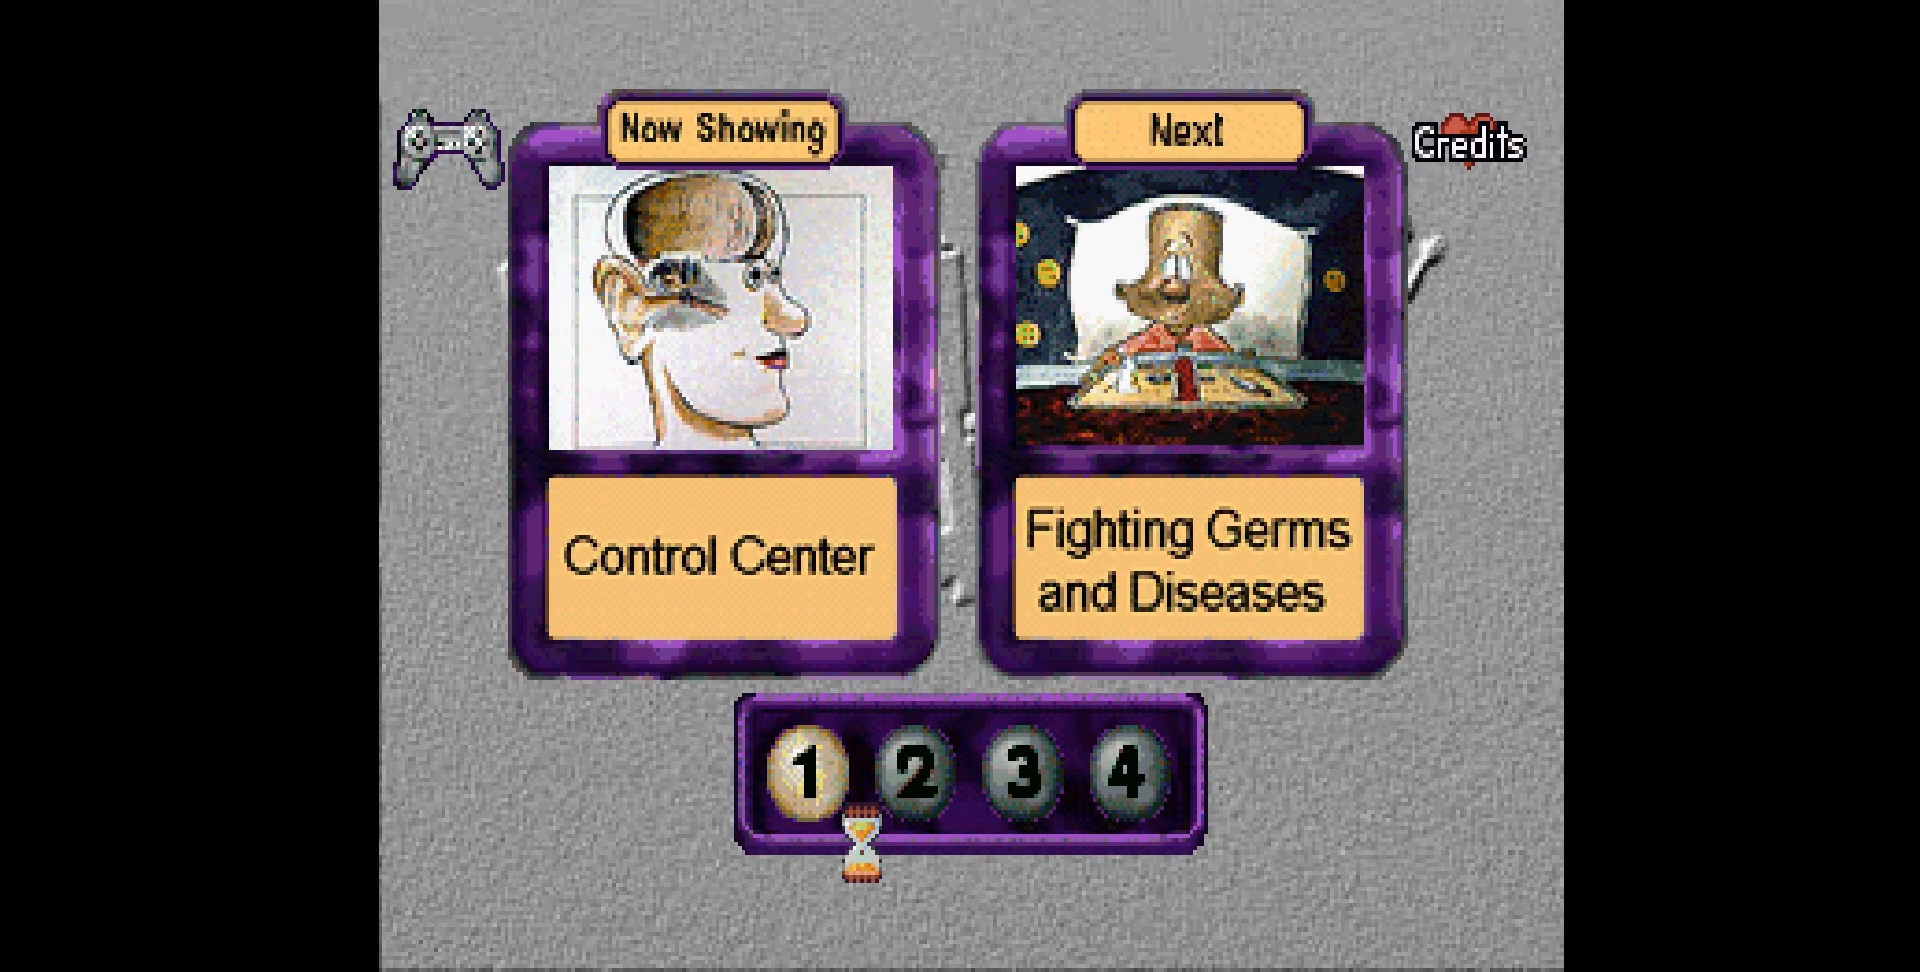
\includegraphics[width=\linewidth]{Games/HeadtoToe/Images/HeadToToe3Image1.png}
        \caption{Head To Toe 3 - Screenshot 1}
    \end{subfigure}
    \begin{subfigure}{0.45\textwidth}
        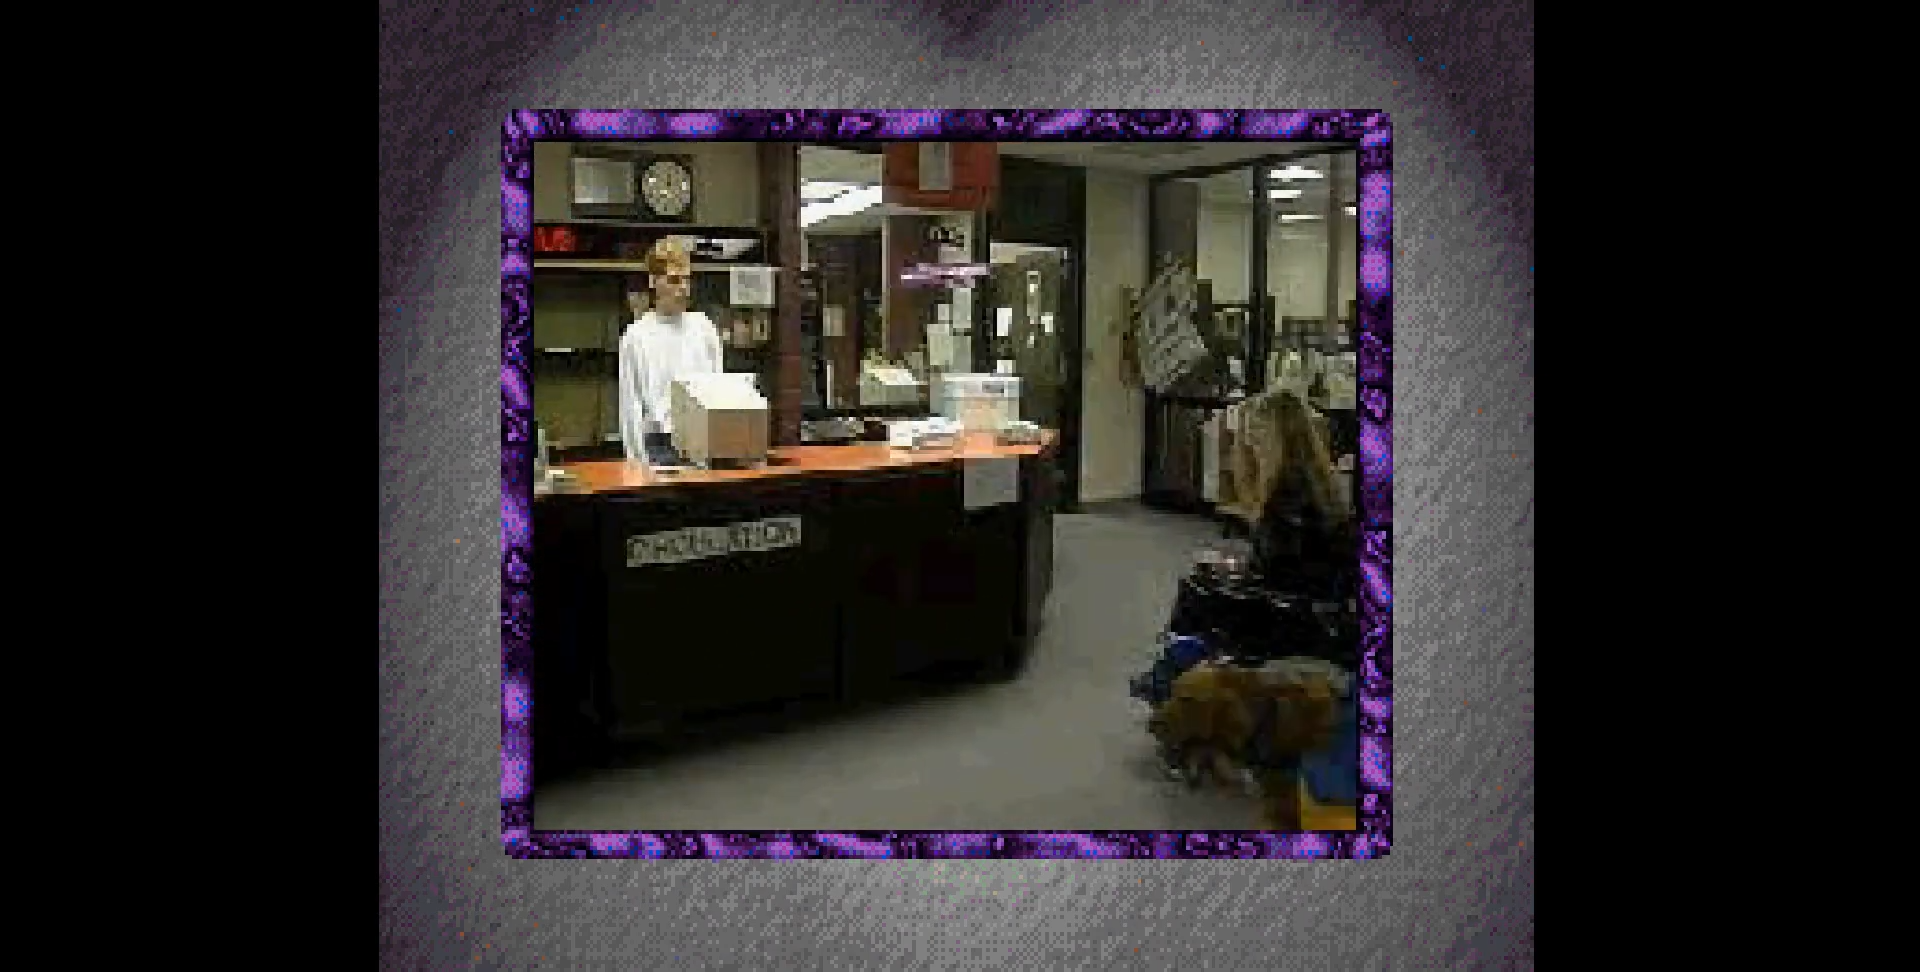
\includegraphics[width=\linewidth]{Games/HeadtoToe/Images/HeadToToe3Image2.png}
        \caption{Head To Toe 3 - Screenshot 2}
    \end{subfigure}

    \begin{subfigure}{0.45\textwidth}
        \centering
        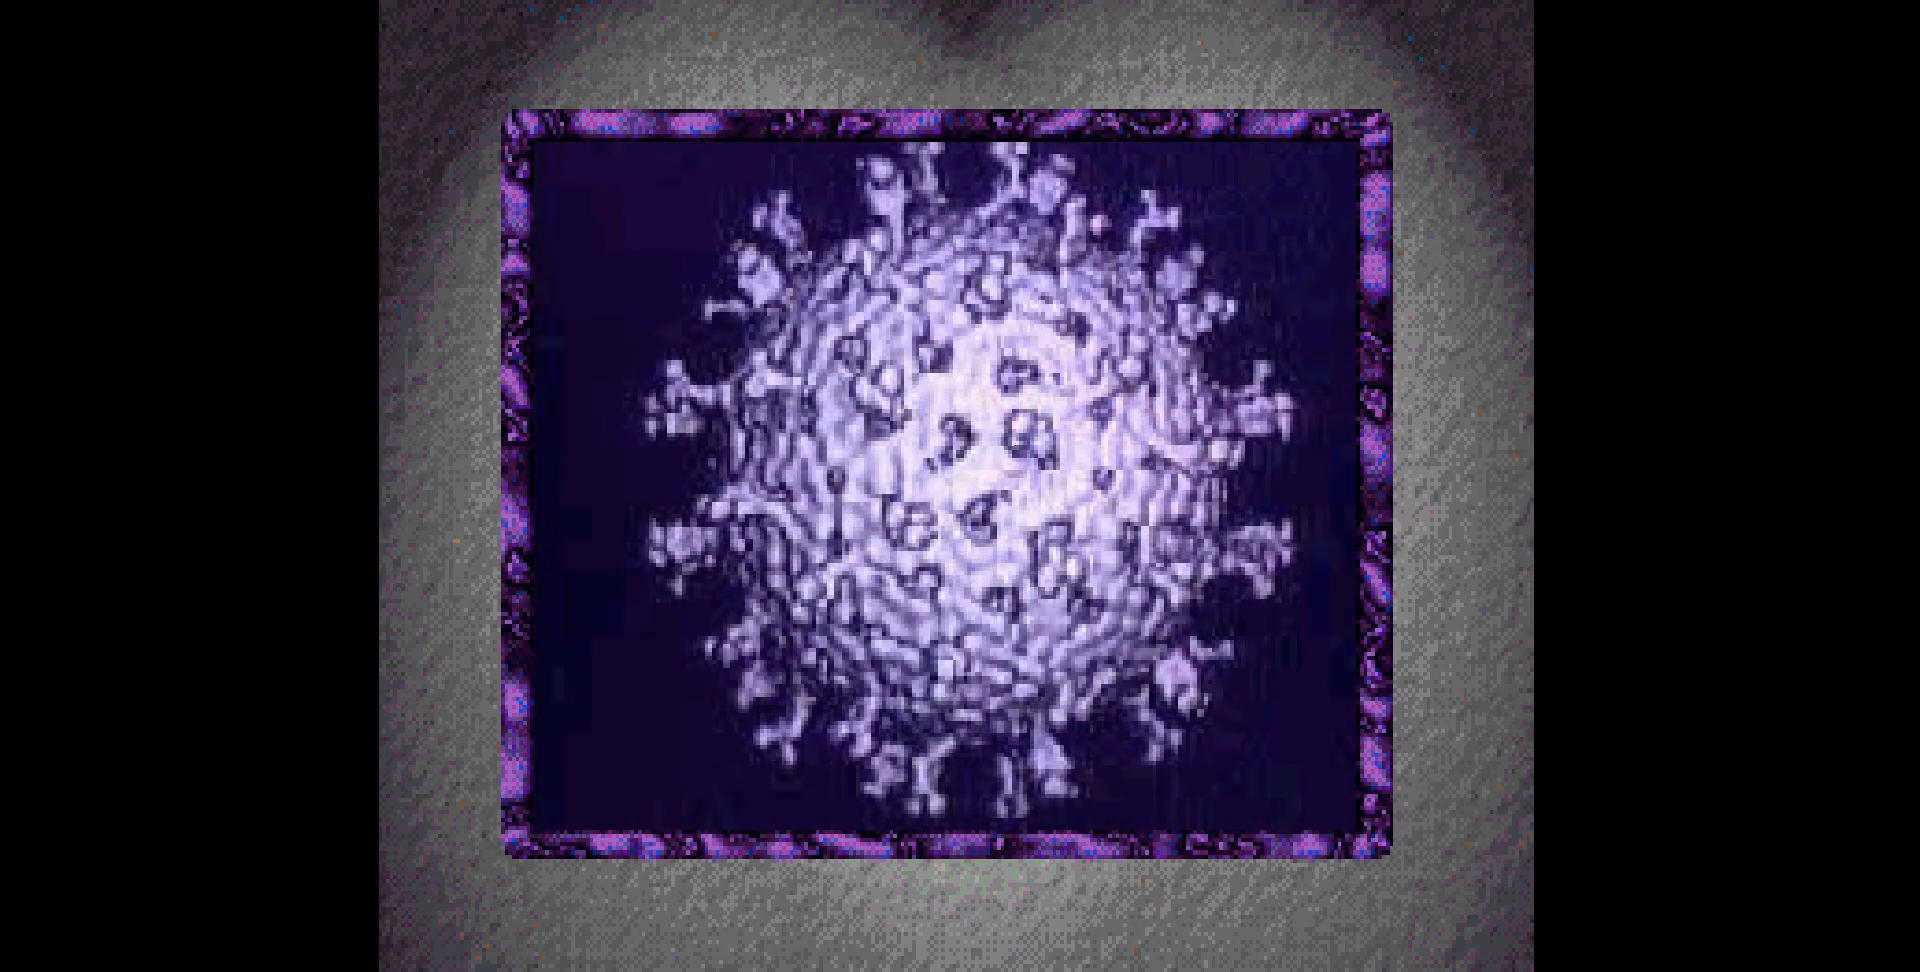
\includegraphics[width=\linewidth]{Games/HeadtoToe/Images/HeadToToe3Image3.png}
        \caption{Head To Toe 3 - Screenshot 3}
    \end{subfigure}
    \begin{subfigure}{0.45\textwidth}
        \centering
        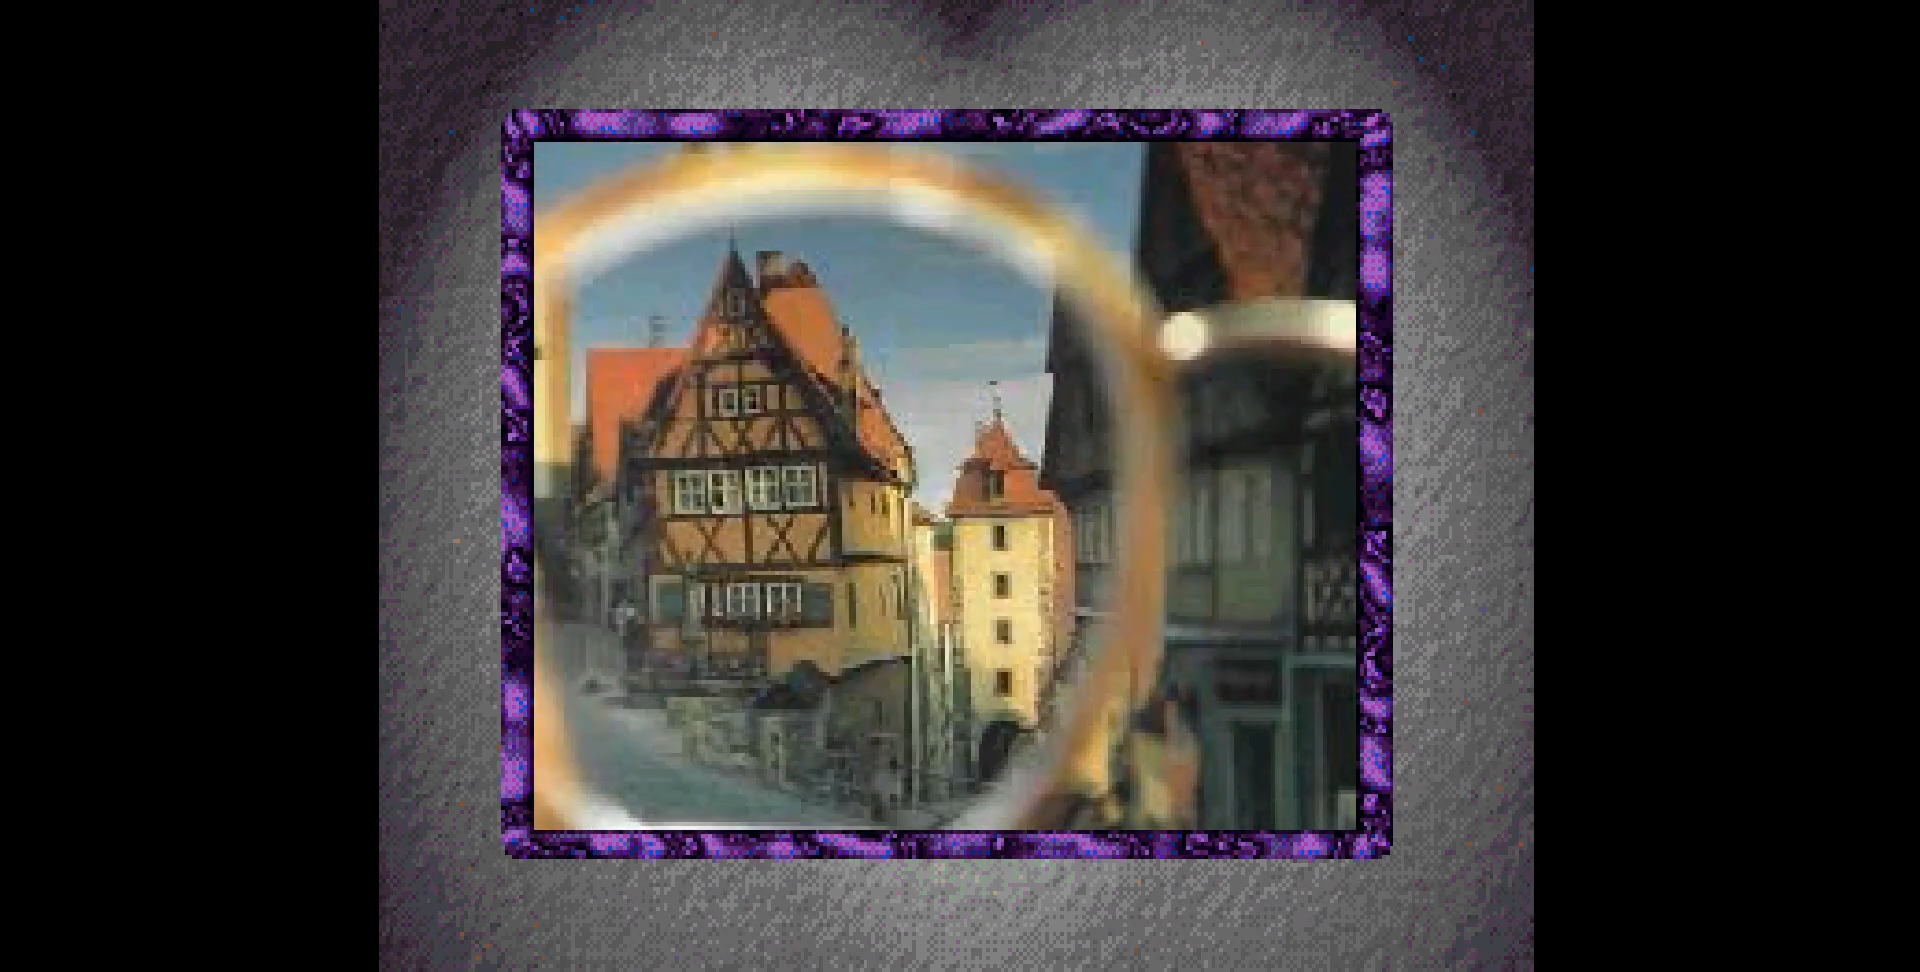
\includegraphics[width=\linewidth]{Games/HeadtoToe/Images/HeadToToe3Image4.png}
        \caption{Head To Toe 3 - Screenshot 4}
    \end{subfigure}
    \caption{Screenshots from Head To Toe 3}
\end{figure}